% =============================================================================
% Section 13: Budget
% =============================================================================

\section{Budget}\label{sec:budget}
\sectionauthors{CM, BS, MN}

\subsection{Budget Overview}

The project budget encompasses both material costs and labor costs, providing a comprehensive view of project investment. Material costs include all electronic components (with a 1.2$\times$ spare parts buffer) and mechanical hardware. Labor costs total 2,888 person-hours across all six team members at a standard rate of \$20 per hour. A 10\% contingency reserve is included to account for unforeseen expenses and scope adjustments.

\begin{table}[H]
\centering
\caption{Budget Summary}
\label{tab:budget_summary}
\begin{tabular}{@{}lr@{}}
\toprule
\textbf{Category} & \textbf{Amount} \\
\midrule
Electronics (w/ 1.2$\times$ Spare Buffer) & \$294.81 \\
Mechanical Components & \$377.25 \\
\midrule
\textbf{Total Material Value} & \textbf{\$672.06} \\
\midrule
Labor Costs (2,888 hours @ \$20/hr) & \$57,760.00 \\
\midrule
Subtotal & \$58,432.06 \\
Reserve (10\%) & \$5,843.21 \\
\midrule
\textbf{Total Project Value} & \textbf{\$64,275.27} \\
\bottomrule
\end{tabular}
\end{table}

\subsection{Material Costs - Bill of Materials}

The Bill of Materials (BOM) details all physical components required for the project. Pricing uses the lowest available price between DigiKey and Mouser for each component. A 1.2$\times$ spare parts buffer (20\% additional) is applied to electronics costs to account for assembly losses and testing. For complete component details including part numbers and supplier links, see Appendix~\ref{app:bom}.

\begin{longtable}{@{}p{0.36\textwidth}rrrp{0.08\textwidth}@{}}
\caption{Bill of Materials: PCB Summary (1.2$\times$ Buffer Applied)} \label{tab:bom} \\
\toprule
\textbf{Board} & \textbf{Parts} & \textbf{Raw Cost} & \textbf{Buffered} & \textbf{Ref} \\
\midrule
\endfirsthead
\multicolumn{5}{c}{\tablename\ \thetable{} (Continued from previous page)} \\
\toprule
\textbf{Board} & \textbf{Parts} & \textbf{Raw Cost} & \textbf{Buffered} & \textbf{Ref} \\
\midrule
\endhead
\midrule
\multicolumn{5}{r}{Continued on next page} \\
\endfoot
\bottomrule
\endlastfoot

\multicolumn{5}{l}{\textbf{Power Management}} \\
3.3V Buck Regulator & 15 & \$7.00 & \$8.40 & \ref{tab:bom-p3v3-full-app} \\
5V Buck Regulator & 23 & \$16.29 & \$19.55 & \ref{tab:bom-p5v0-full-app} \\
6V Buck Regulator & 34 & \$37.78 & \$45.34 & \ref{tab:bom-p6v0-full-app} \\
\addlinespace

\multicolumn{5}{l}{\textbf{Battery Management}} \\
Analog Front-End (AFE) & 81 & \$37.91 & \$45.49 & \ref{tab:bom-afe-full-app} \\
Buck-Boost Charger & 43 & \$17.51 & \$21.01 & \ref{tab:bom-charger-full-app} \\
Fuel Gauge & 46 & \$15.18 & \$18.22 & \ref{tab:bom-fuel-full-app} \\
Gate Driver & 12 & \$5.03 & \$6.04 & \ref{tab:bom-gate-full-app} \\
\addlinespace

\multicolumn{5}{l}{\textbf{Control/Interface}} \\
LiDAR Breakout & 5 & \$11.15 & \$13.38 & \ref{tab:bom-lidar-full-app} \\
MCU Board & 42 & \$53.83 & \$64.60 & \ref{tab:bom-mcu-full-app} \\
Motor Driver & 42 & \$28.39 & \$34.07 & \ref{tab:bom-motor-full-app} \\
USB-C PD Controller & 51 & \$15.59 & \$18.71 & \ref{tab:bom-usbc-full-app} \\
\addlinespace

\midrule
\textbf{Electronics Subtotal} & \textbf{394} & \textbf{\$245.66} & \textbf{\$294.81} & \\
\addlinespace
\multicolumn{5}{l}{\textbf{Mechanical Components}} \\
Chassis, Motors, Hardware & -- & -- & \$377.25 & \ref{tab:bom-mechanical} \\
\addlinespace
\midrule
\textbf{Total Material Value} & & & \textbf{\$672.06} & \\
\end{longtable}

\subsection{Material Costs by Category}

\begin{table}[H]
\centering
\caption{Material Value Distribution by Category}
\label{tab:material_by_category}
\begin{tabular}{@{}lrrr@{}}
\toprule
\textbf{Category} & \textbf{Raw Cost} & \textbf{With Buffer} & \textbf{Percentage} \\
\midrule
Power Management & \$61.07 & \$73.29 & 10.9\% \\
Battery Management & \$75.63 & \$90.76 & 13.5\% \\
Control/Interface & \$108.96 & \$130.76 & 19.5\% \\
Mechanical & \$377.25 & \$377.25 & 56.1\% \\
\midrule
\textbf{Total} & \textbf{\$622.91} & \textbf{\$672.06} & \textbf{100\%} \\
\bottomrule
\end{tabular}
\end{table}

\subsection{Labor Costs}

Labor costs are calculated based on team member effort allocation at a standard rate of \$20 per hour. Hours are derived from the Work Breakdown Structure activities, with each person-day representing 8 hours of effort:

\begin{table}[H]
\centering
\caption{Labor Cost by Team Member}
\label{tab:labor_costs}
\begin{tabular}{@{}lrrr@{}}
\toprule
\textbf{Team Member} & \textbf{Hours} & \textbf{Rate} & \textbf{Cost} \\
\midrule
Cesar Magana (CM) & 768 & \$20/hr & \$15,360.00 \\
Jeremie Hews (JH) & 592 & \$20/hr & \$11,840.00 \\
Jared Bartz (JB) & 488 & \$20/hr & \$9,760.00 \\
Shawn Ciaciura (SC) & 368 & \$20/hr & \$7,360.00 \\
Brighton Sikarskie (BS) & 352 & \$20/hr & \$7,040.00 \\
Michael Norton (MN) & 320 & \$20/hr & \$6,400.00 \\
\midrule
\textbf{Total Labor} & \textbf{2,888} & & \textbf{\$57,760.00} \\
\bottomrule
\end{tabular}
\end{table}

\subsection{Monthly Budget Breakdown}

The following table shows planned expenditures by month, aligned with the five project phases (Research, Design, Build, Test, Close). Material purchases are concentrated in the Build phase when components are ordered, while labor costs follow the activity schedule:

\begin{table}[H]
\centering
\caption{Monthly Budget Distribution}
\label{tab:monthly_budget}
\begin{tabular}{@{}llrrr@{}}
\toprule
\textbf{Month} & \textbf{Phase} & \textbf{Materials} & \textbf{Labor} & \textbf{Total} \\
\midrule
Aug 2025 & Research & \$0.00 & \$320.00 & \$320.00 \\
Sep 2025 & Research & \$0.00 & \$4,320.00 & \$4,320.00 \\
Oct 2025 & Research & \$0.00 & \$5,120.00 & \$5,120.00 \\
Nov 2025 & Design & \$25.00 & \$8,640.00 & \$8,665.00 \\
Dec 2025 & Design & \$25.00 & \$5,280.00 & \$5,305.00 \\
Jan 2026 & Design/Build & \$200.00 & \$6,400.00 & \$6,600.00 \\
Feb 2026 & Build & \$250.00 & \$8,000.00 & \$8,250.00 \\
Mar 2026 & Build/Test & \$122.06 & \$7,840.00 & \$7,962.06 \\
Apr 2026 & Test & \$50.00 & \$8,000.00 & \$8,050.00 \\
May 2026 & Test/Close & \$0.00 & \$3,840.00 & \$3,840.00 \\
\midrule
\textbf{Total} & & \textbf{\$672.06} & \textbf{\$57,760.00} & \textbf{\$58,432.06} \\
\bottomrule
\end{tabular}
\end{table}

\subsection{Budget Visualization}

\cref{fig:budget_chart} illustrates the budget distribution across material categories. The pie chart shows the relative allocation by subsystem, while the bar chart displays per-board costs with the 1.2$\times$ buffer applied.

\begin{figure}[H]
\centering
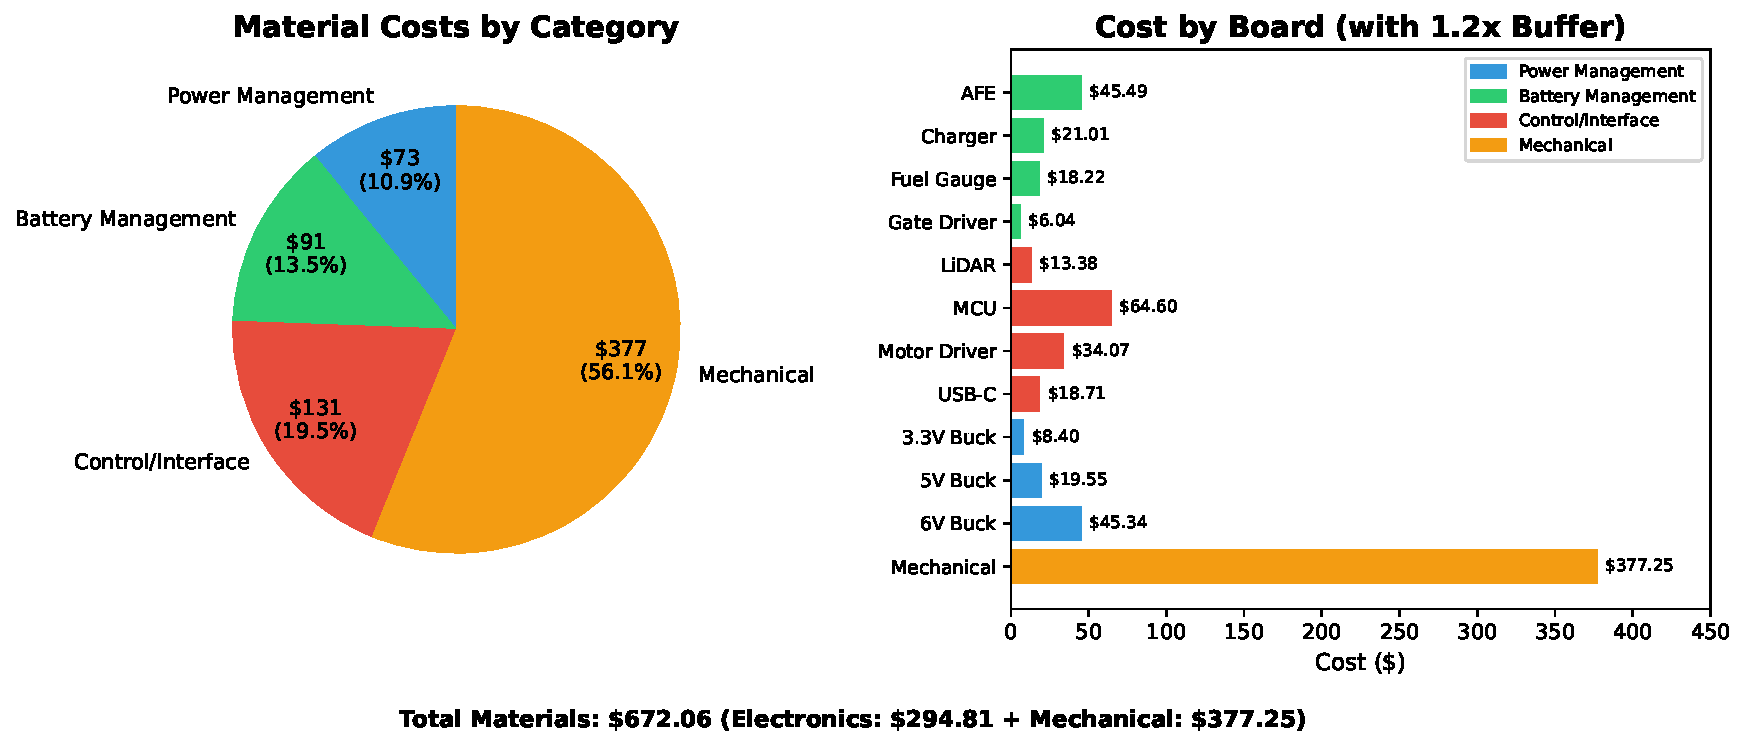
\includegraphics[width=0.9\textwidth]{figures/budget_static.pdf}
\caption{Budget Distribution by Category and Board}
\label{fig:budget_chart}
\end{figure}

\subsection{Contingency Reserve}

A 10\% contingency reserve (\$5,843.21) is allocated to address:

\begin{itemize}
    \item Component price fluctuations or supply chain delays
    \item Design iterations requiring additional materials
    \item Scope adjustments approved through change control
    \item Unforeseen testing or integration requirements
\end{itemize}

\noindent The reserve is managed under strict change control and requires Project Manager approval for any withdrawals.
